\documentclass[notes=hide,yellow]{beamer}

% (c) 2008 Steffen Klemer <moh AT gmx BEEP org>
% This work is licensed under the Creative Commons Attribution-Share Alike 3.0
% Germany License. To view a copy of this license, visit
% http://creativecommons.org/licenses/by-sa/3.0/de/ or send a letter to Creative
% Commons, 171 Second Street, Suite 300, San Francisco, California, 94105, USA.
%
% See http://www.noch-mehr-davon.de/vortr.shtml
% Permissions beyond the scope of this license may be available at the same site
%
% Template based on: Copyright 2004 by Till Tantau <tantau@users.sourceforge.net>.


\mode<presentation>
{
%	\usetheme{AnnArbor} %Szeged
%	\usetheme{Berkeley}
	\usetheme{Dresden}
%	\usecolortheme{rose} %oder beaver oder rose oder orchid, albatross, rose
% 	\useinnertheme{circles}
%	\useoutertheme{split}
%	\setbeamercovered{invisible} %or transparent
% 	\usefottheme{professionalfonts}
% 	\usefonttheme[onlymath]{serif}
        %\setbeamercovered{invisible}
%	\setbeamertemplate{navigation symbols}{}
}

\usepackage{amsmath,amssymb,latexsym}
\usepackage{fancyvrb}
\usepackage{graphicx}
\usepackage{epstopdf}
\usepackage{amsfonts}
\usepackage{amsthm}
\usepackage{wasysym}
\usepackage{ucs}
\usepackage{listings}
\usepackage{stmaryrd}
\usepackage{hyperref}
\usepackage{graphics}
\usepackage{colortbl}
\usepackage[ngerman]{babel}
\usepackage[utf8x]{inputenc}
\usepackage{tikz}
\usepackage[numbers,sort&compress]{natbib}



\tikzstyle{every picture}+=[remember picture]
\usetikzlibrary{arrows}
\usetikzlibrary{shadows}
\usetikzlibrary{fit}
\usetikzlibrary{shapes}
\usetikzlibrary{backgrounds}

\tikzstyle{vertex}=[circle,fill=black!25,minimum size=12pt,inner sep=0pt]
\tikzstyle{selected vertex} = [vertex, fill=red!24]
\tikzstyle{blue selected vertex} = [vertex, fill=blue!25]
\tikzstyle{edge} = [draw,thick,-]
\tikzstyle{weight} = [font=\small]
\tikzstyle{selected edge} = [draw,line width=5pt,-,red!50]
\tikzstyle{ignored edge} = [draw,line width=5pt,-,black!20]
\tikzstyle{small vertex}=[circle,fill=black!25,minimum size=8pt, inner sep=0pt]
\tikzstyle{small selected vertex}=[circle,fill=red!25,minimum size=8pt, inner sep=0pt]







\title{Das verteilte Filesystem Ceph als Storage-Lösung}
\subtitle{ }
\author{Ralph Krimmel}



\begin{document}
	\nocite{*} 
	\begin{frame}
		\titlepage
	\end{frame}

	\begin{frame}
		\tableofcontents
	\end{frame}


\section{Einf\"uhrung}
\subsection*{}

\begin{frame}{Motivation}

\begin{itemize}
	\item Institut f\"ur Numerische und Angwandte Mathematik
	\item \textasciitilde 50 Mitarbeiter
	\item Hardware: 10 inhomogene Server
	\item Kein SAN
	\item Dienste (schon teilweise virtualisiert)
	\begin{itemize}
		\item Fileserver
		\item Webserver
		\item Email \& Groupware
		\item Jabber
		\item Diverse Lizenzserver
		\item Versionsverwaltung (svn, git, hg)
		\item ...
	\end{itemize}
\end{itemize}
\end{frame}

\begin{frame}{Probleme}

	\begin{itemize}
		\item Fileserver
			\begin{itemize}
				\item Dateisystem: ZFS 
				\item Netzwerkdateisystem: NFS
				\item \glqq Hot spare Replikation\grqq 
				\item $\Rightarrow$ Nadel\"ohr
			\end{itemize} 
		\item <2> Restliche Server
			\begin{itemize}
				\item Unbenutzte Speicherkapazit\"at
				\item Unbenutzte Rechenapazit\"at
				\item Unzureichende Verf\"ugbarkeit bei Fehlern
			\end{itemize}
	\end{itemize}
\end{frame}

\begin{frame}{Fileserver Availability}
	\begin{center}
	\includegraphics[width=0.65\textwidth]{availabilitysuitenew.jpg}
	\end{center}
	\small
	Quelle: \texttt{http://hub.opensolaris.org/bin/view/Project+avs/}
\end{frame}


\begin{frame}{L\"osungsansatz}
	
	\begin{itemize}
		\item Jeder Server wird Hypervisor
		\item Verteiltes Dateisystem 
	%		\begin{itemize}
	%			\item Ausfalltoleranz (Verf\"ugbarkeit und Zuverl\"assigkeit) durch Replikation
	%			\item Hohe Performanz durch Striping %Aufteilen der Daten auf mehrere physikalische Devices
	%		\end{itemize}
		\item <2> Buzzword: \glqq Private Cloud\grqq
	\end{itemize}

\end{frame}

\begin{frame}{Definition}
		In computing, a distributed file system or network file system is any file system that allows access to files from multiple hosts via a computer network.$[1]$
	\tiny{$[1]$ Galvin Silberschatz (1994). Operating System concepts, chapter 17 Distributed file systems. Addison-Wesley Publishing Company.} \\ 
\end{frame}

\begin{frame}{Nichts neues...}

		z.B. NFS, entwickelt von Sun Microsystems in 1984
		\begin{center}
			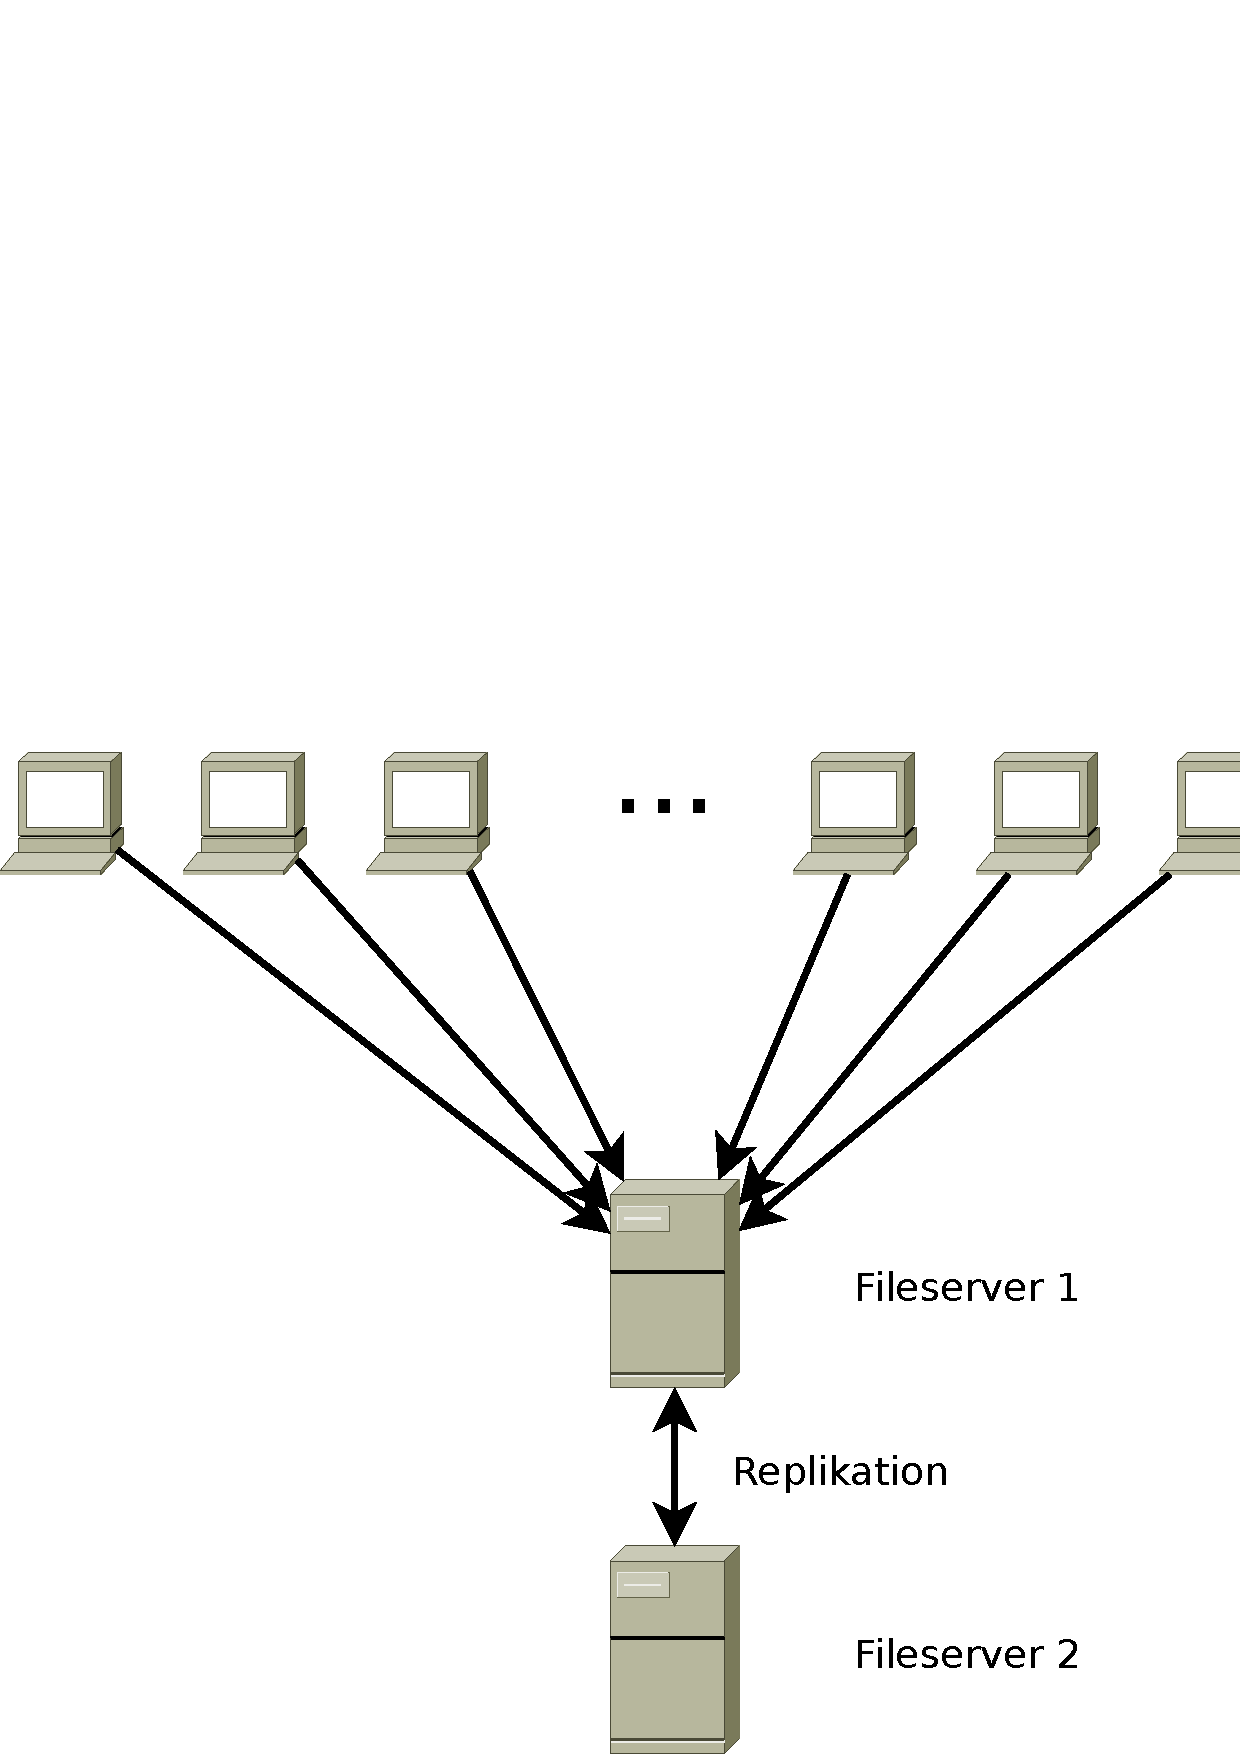
\includegraphics[scale=0.2]{nfs.pdf}
		\end{center}
		\begin{itemize}
			\item Schlechte Performanz bei vielen Clients \\ $\Rightarrow$ Skaliert nicht
			\item Keine Fehlertoleranz
		\end{itemize}
\end{frame}



\begin{frame}{Anforderungen an ein modernes, verteiltes Dateisystem}
%	\begin{block}{Anforderungen}
	\begin{itemize}
		\item Hohe Performanz durch Striping
			\begin{itemize}
				\item Durchsatz
				\item Latenz
			\end{itemize}
		\item Skalierbarkeit
		\item Verf\"ugbarkeit
		\item Zuverl\"assigkeit
	\end{itemize}
%	\end{block}
\end{frame}

\begin{frame}{Zuverl\"assigkeit/Verf\"ugbarkeit}
	Problem: Fehler sind mehr die Norm als die Ausnahme
	\begin{itemize}
		\item System g\"unstiger Hardware
		\item Fehler in Programmen %theres software that always crashes 
		\item Menschliches Versagen % what was this cable for?
		\item Betriebssystemfehler % ever used windows?
		\item Ausfall von: 
		\begin{itemize}
			\item Festplatten
			\item Arbeitsspeicher
			\item Kabel
			\item Netzwerk
			\item ...
		\end{itemize}
	\end{itemize}		
\end{frame}

\begin{frame}{Moderner Ansatz}
	\begin{itemize}
		\item Objektbasiert
		\item Festplatten $\rightarrow$ Intelligent object storage devices (OSD's)
		\begin{itemize}
			\item CPU
			\item Netzwerkschnittstelle
			\item Lokaler Cache
		\end{itemize}
		\item Metadaten getrennt von Nutzdaten
	\end{itemize}
\end{frame}


\begin{frame}{Typischer Zugriff (z.B. Hadoop)}
	\begin{center}
	\includegraphics[scale=0.2]{hdfsarchitecture.jpg}
	\end{center}
	\small
	Quelle: \texttt{http://hadoop.apache.org/common/docs/r0.20.2/hdfs\_design.html}
\end{frame}




\section{Ceph - Theorie}
\subsection*{}
\begin{frame}
	\begin{center}
		\includegraphics{ceph_architecture.pdf}
	\end{center}
	Quelle: \cite{weil2006}
\end{frame}


\begin{frame}

\end{frame}


\section{Ceph - Praxis}
\subsection*{}
\begin{frame}

\end{frame}

\section{Fragen}
\subsection*{}
\begin{frame}
	\begin{center}
	\large Questions?
	\end{center}
	
	\begin{center}
	\includegraphics[scale=0.8]{questions.jpg}
	\end{center}
\end{frame}

\begin{frame}{Literatur}
	\bibliographystyle{apalike}
	\bibliography{literature}	
\end{frame}

\end{document}


